\chapter{任务二:发音与听觉感知}
\label{chap:task2}

\section{语音的谐波 harmonics}
从波形图中我们很难看出语音的谐波分量,不过我们可以通过语谱图轻松地看出语音的谐波及其能量。

\section{比较 EGG 和语音信号波形}
在图~\ref{fig:waveforms_speech_EGG}中展示了语音信号波形和 EGG 信号波形的示例。
首先,EGG 和语音信号的时间长度是一样的,并且他们的清音和浊音的区域是一致的。
其次,音高(基频 $F_0$) 是一致的,虽然从波形图中无法直接看出来。

\begin{figure}[htp]
    \subfloat[语音信号波形]{%
        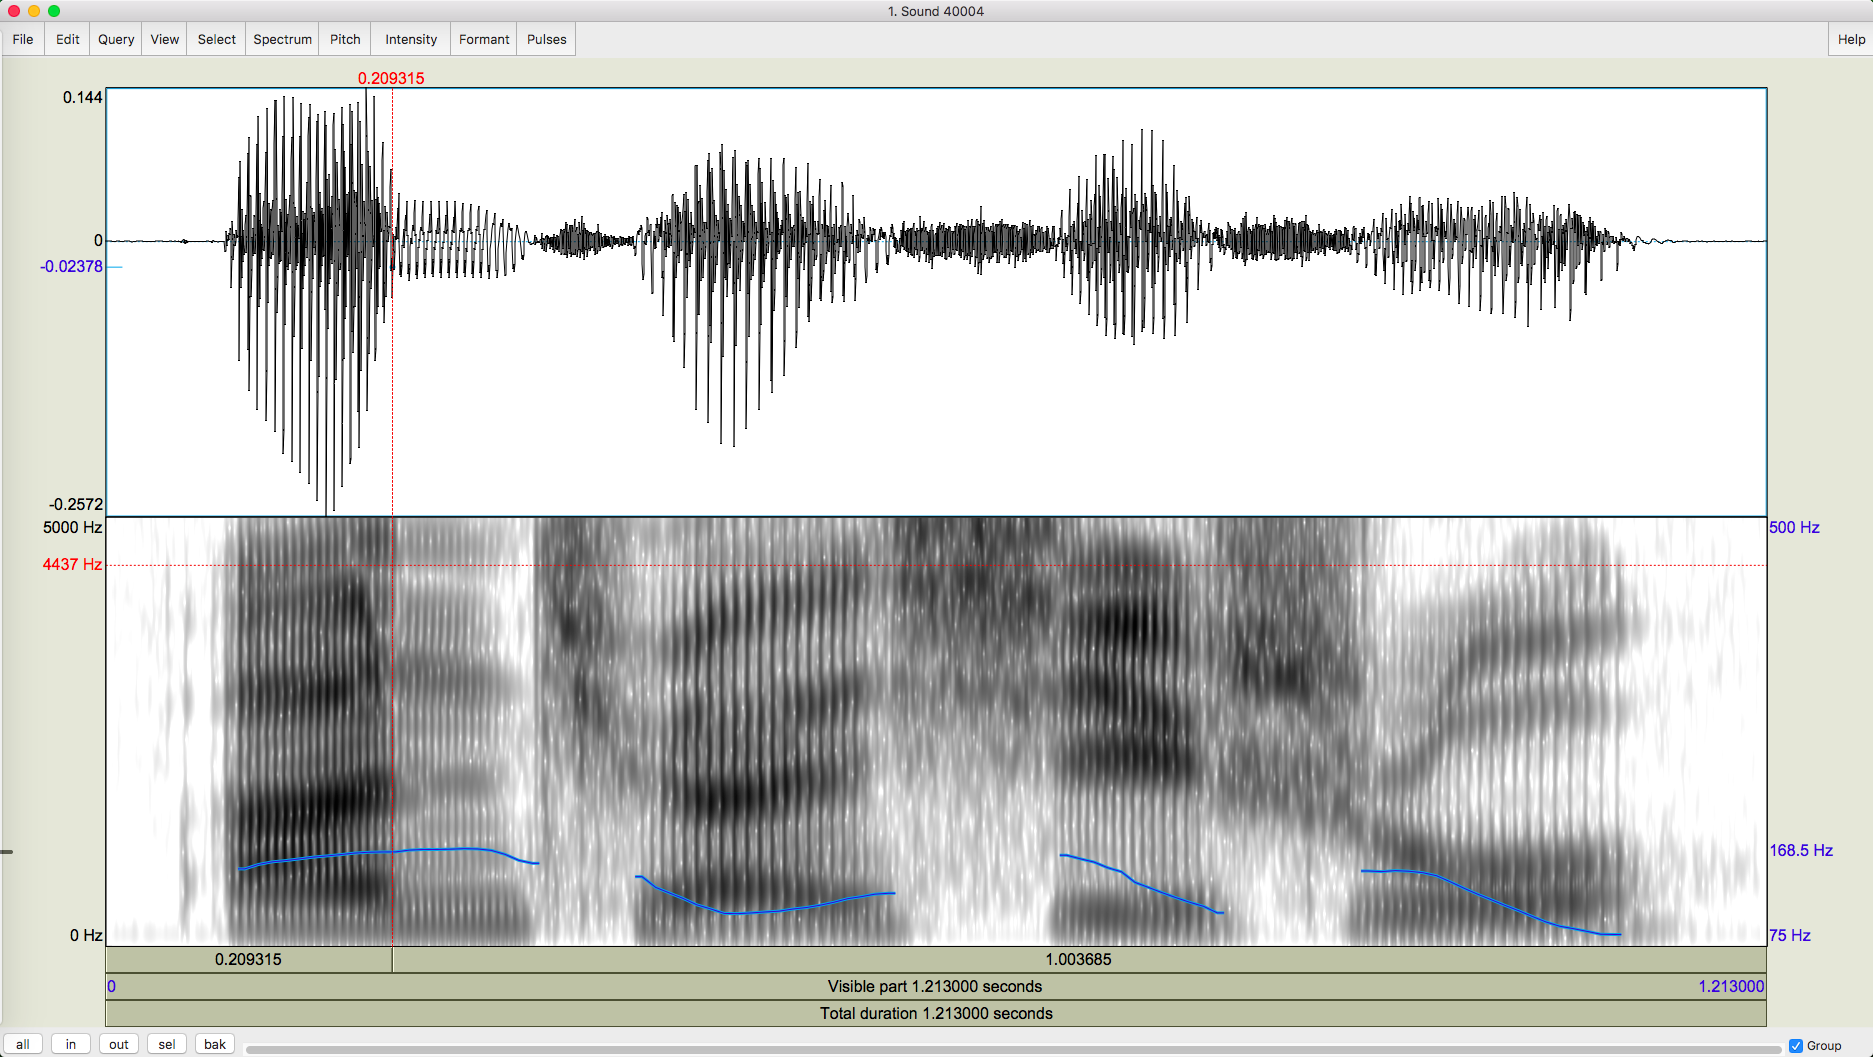
\includegraphics[clip,width=\columnwidth]{waveform_speech.png}%
    }
    \subfloat[EGG信号波形]{%
        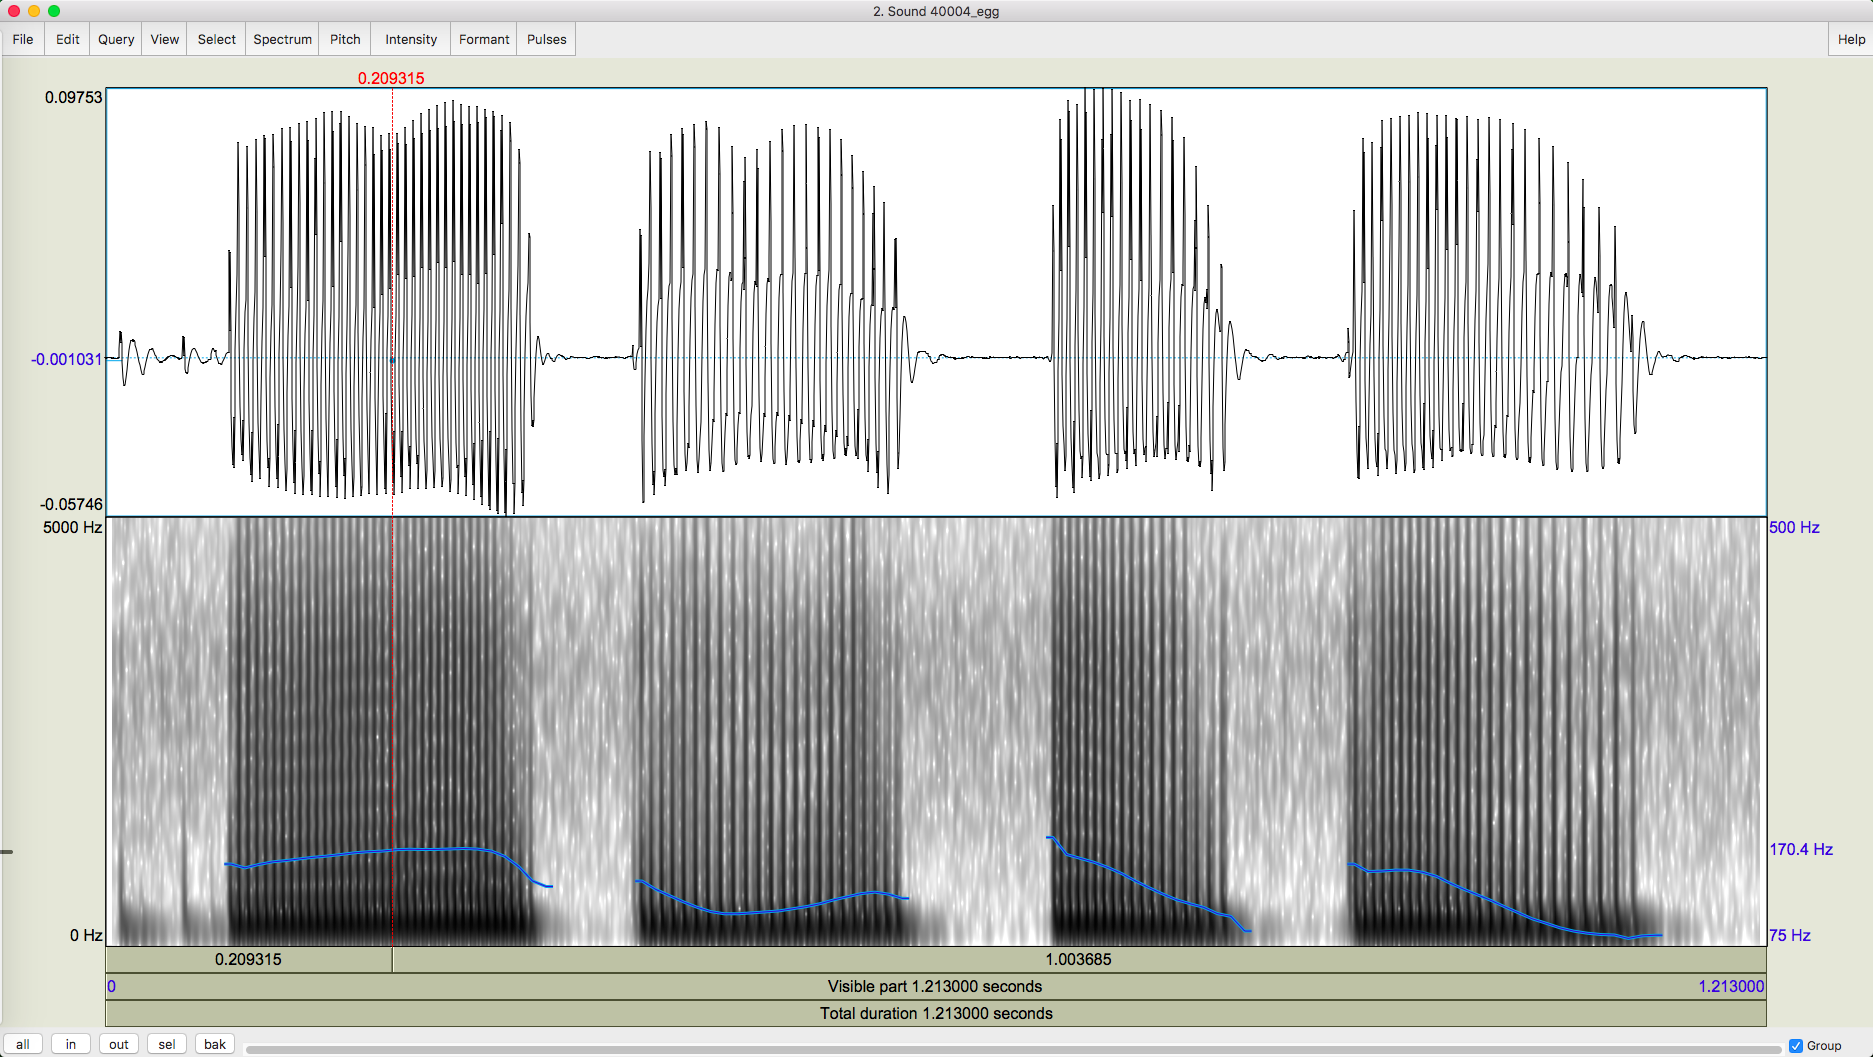
\includegraphics[clip,width=\columnwidth]{waveform_EGG.png}%
    }
    \caption{比较 EGG 和语音信号波形}
    \label{fig:waveforms_speech_EGG}
\end{figure}

不同点在于,语音信号是 EGG 经过声道调制(Filter)后的输出。
EGG 信号在同一段浊音内表现出来的波形是比较规整的谐波信号。
具有较明显的周期性,也就是说其振幅的局部最大值的抖动较小。
并且对于清音部分,其能量很小,而且波动幅度也很小,说明噪声比较微弱。
其语谱图中的能量也是从基频到谐波分量,随着频率增加,能量逐渐下降。

而语音信号表现为其抖动更加明显,并且在大时间尺度上没有明显的周期性,而在很小一段时间内其信号具有比较明显的周期性。
并且对于清音部分,可以明显看出其能量和波动都比 EGG 明显,说明噪声比较大。
从语谱图中我们可以看到,各个频率的能量分布与频率大小关系不大,不过具有比较明显的峰值特性,也就是说,语谱图中某一部分区域的能量比较大,而其他地方能量比较小,看起来有点像山峰山谷。

\section{不同情绪的基音轮廓}
可以从图中看出:

\begin{enumerate}
    \item 中性情绪的基音轮廓比较平滑,变化幅度不会很大。浊音和清音(没有基音轮廓的部分)的识别较好,间断点较少。
    \item 愤怒情绪的基音轮廓抖动比较大,有些部分浊音被错误识别为了清音,所以基音轮廓有更加多的间断点。同时,可以看出,其平均的基音频率都要高于中性情绪。听该段音频的时候明显感觉声音起伏落差明显,而且很急促。
    \item 悲伤情绪的基音轮廓抖动同样也比较大,也有一部分浊音被错误识别为清音的情况,不过间断点略少于愤怒情绪。同样的,其平均基音频率要低于中性情绪,而且听的时候也明显感觉声音要低沉很多。
\end{enumerate}

\section{不同语气的基音轮廓}

\section{宽带语谱图和窄带语谱图}

\section{掩蔽效应}